% -*- mode: latex; -*- mustache tags:  
\documentclass[10pt,twoside,english]{_support/latex/sbabook/sbabook}
\let\wholebook=\relax

\usepackage{import}
\subimport{_support/latex/}{common.tex}

%=================================================================
% Debug packages for page layout and overfull lines
% Remove the showtrims document option before printing
\ifshowtrims
  \usepackage{showframe}
  \usepackage[color=magenta,width=5mm]{_support/latex/overcolored}
\fi


% =================================================================
\title{Learning Object-Oriented Programming, Design and TDD with Pharo}
\author{Stéphane Ducasse}
\series{The Pharo TextBook Collection}

\hypersetup{
  pdftitle = {Learning Object-Oriented Programming, Design and TDD with Pharo},
  pdfauthor = {Stéphane Ducasse},
  pdfkeywords = {Introduction, programming, design, testing, Pharo, Smalltalk}
}


% =================================================================
\begin{document}

% Title page and colophon on verso
\maketitle
\pagestyle{titlingpage}
\thispagestyle{titlingpage} % \pagestyle does not work on the first one…

\cleartoverso
{\small

  Copyright 2017 by Stéphane Ducasse.

  The contents of this book are protected under the Creative Commons
  Attribution-ShareAlike 3.0 Unported license.

  You are \textbf{free}:
  \begin{itemize}
  \item to \textbf{Share}: to copy, distribute and transmit the work,
  \item to \textbf{Remix}: to adapt the work,
  \end{itemize}

  Under the following conditions:
  \begin{description}
  \item[Attribution.] You must attribute the work in the manner specified by the
    author or licensor (but not in any way that suggests that they endorse you
    or your use of the work).
  \item[Share Alike.] If you alter, transform, or build upon this work, you may
    distribute the resulting work only under the same, similar or a compatible
    license.
  \end{description}

  For any reuse or distribution, you must make clear to others the
  license terms of this work. The best way to do this is with a link to
  this web page: \\
  \url{http://creativecommons.org/licenses/by-sa/3.0/}

  Any of the above conditions can be waived if you get permission from
  the copyright holder. Nothing in this license impairs or restricts the
  author's moral rights.

  \begin{center}
    
\includegraphics[width=0.2\textwidth]{_support/latex/sbabook/CreativeCommons-BY-SA.pdf}
  \end{center}

  Your fair dealing and other rights are in no way affected by the
  above. This is a human-readable summary of the Legal Code (the full
  license): \\
  \url{http://creativecommons.org/licenses/by-sa/3.0/legalcode}

  \vfill

  % Publication info would go here (publisher, ISBN, cover design…)
  Layout and typography based on the \textcode{sbabook} \LaTeX{} class by Damien
  Pollet.
}


\frontmatter
\pagestyle{plain}

\tableofcontents*
\clearpage\listoffigures

\mainmatter

\chapter{About this book }\label{ch:about}\section{A word of presentation}
I started to write this book back in 1998 when I wrote around 900 pages in preparation for \textit{Learning Programming with Robots}
(Apparently, I needed to write to understand what I wanted to explain and how). From this I extracted \textit{Learning Programming with Robots}, which was a book to teach simple concepts such as variables, loops, procedures and to help people teach kids how to program. My original objective was to write a second volume to teach object-oriented programming. But while this first volume was a success, I got really frustrated because to be understandable by everyone I had to remove what I like: object-oriented programming and good object-oriented design. 

At that time, I met Harald Wertz, who gave me really nice ideas and pointers such as L-systems, then asked why I focused on procedural thinking and suggested that I should teach object-oriented programming instead. And he was right. This remark was like a bee in my bonnet for more than ten years.
In fact, it was my original objective but I was exhausted after my first attempt and I had to focus on my academic life.

Now, nearly fifteen years later, I'm ready to write a book to start with object-oriented programming. In fact, I rewrote everything I got from that time. 
I hope that you will enjoy it as much as I did — even if, for me, writing a book is a really long and daunting task because I want to make it great.
I plan to write another volume on patterns of design that will extend this book.
\section{Structure of the book}
While writing this book, I faced a challenge to find the correct level of difficulty.
To solve this problem, I structured the book either into key chapters on basic concepts, or into projects on more advanced topics.
The projects are little tutorials or more realistic examples, with step by step explanations; you can skip over them and come back to read them whenever you feel like it.
I also propose various paths through the book with different levels of reading; however, many of the \textit{simpler} chapters also contain design remarks.


\begin{figure}

\begin{center}
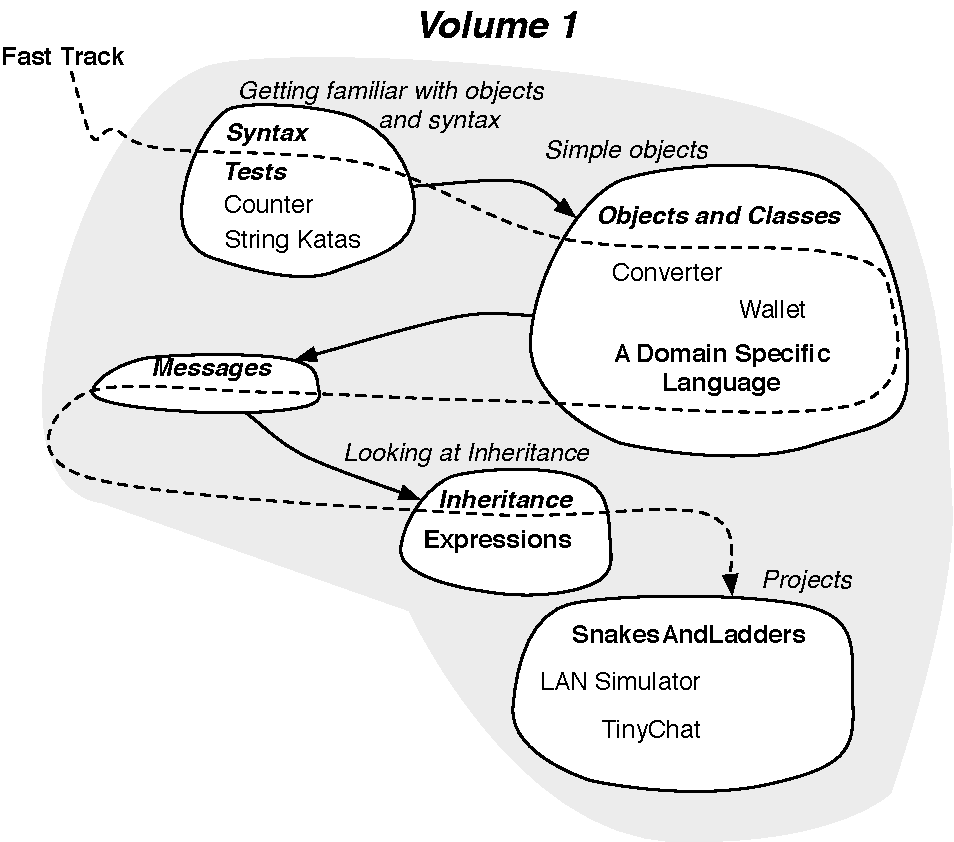
\includegraphics[width=1.0\textwidth]{/Users/ducasse/Workspace/FirstCircle/MyBooks/Bk-Writing/PharoBooks/LearningOOPWithPharoTrans/_result/pdf/Chapters/Introduction/figures/MapVolume1.pdf}\caption{Reading maps.\label{fgmap}}\end{center}
\end{figure}

\subsection{Fast track}
The following chapters contain more conceptual information:

In the volume 1:

\begin{itemize}
\item Glimpse of the syntax
\item Tests, tests and tests
\item Objects and classes
\item Revisiting objects and classes
\item Domain specific language
\item Inheritance and expressions
\item Sending messages
\item Snakes and ladders
\end{itemize}

The other chapters are more exercise and practical. For example, with TinyChat, you will have fun with a web server written in the single page of code. You will find the solutions of the exercises in a separate pdf available on the book web site at \url{http://books.pharo.org} and the associated github repository \url{https://github.com/SquareBracketAssociates/LearningOOPWithPharo}.
\section{What you will learn}
I would like to present the concepts that I want to teach you and that hopefully you should acquire. What is key to understand is that I will focus on the \textit{key} conceptual elements. It is easy for me because I will not explain OOP/D in general but within the context of Pharo and Pharo is the essence of Object-Oriented programming since its object model is minimal but it covers the key and essential aspect of OOP. For example, we will not present method modifiers, types, or overloading (which is a bad concept).

We will focus on object-oriented \textit{programming} concepts:

\begin{itemize}
\item Objects / Classes 
\item Messages / Methods
\item \textcode{self} and its semantics
\item Inheritance
\item \textcode{super} and its semantics
\end{itemize}

…and on object-oriented \textit{design} concepts:

\begin{itemize}
\item Class responsibility collaboration
\item Delegation
\item Message sends are choice
\item Message sends are plans for reuse
\item The \symbol{34}Don't ask, tell\symbol{34} Principle
\item Tests are your life insurance
\item Polymorphism
\end{itemize}

In addition, we will also present 

\begin{itemize}
\item Tests
\item Software refactorings
\end{itemize}
\subsection{Growing software}
Often books present a problem and its solution. Now for non-trivial problems, the solution does not fall from the sky or get developed in one stroke, but it is the constant evolution of a first solution that evolves over time. Such an evolution is often difficult and tedious because the developer jumps from one stable state to a situation where his code may not work anymore. This is where Test Driven Design and refactorings really help.
Test Driven Design helps focusing on new features and captures them as executable entities: tests. Refactorings help by transforming code without breaking its invariants.
Note that tests do not forbid to break code, they help identifying when previous invariants or constraints got violated. Sometimes violated tests identify a bug, but they may be broken just because the requirements changed and that the tests should be updated. 
In this book, I wanted to see how software grows in little steps. This is what I do frequently during my coding sessions, and I think that this is important, to cover the hidden paths in software creation.
\subsection{Syntax, blocks and iterators}
Since we need a language to express our programs, we will teach you the syntax of Pharo. In particular, we will use some simple chapters to get you started. 

Now in a nutshell, you should know that the Pharo syntax

\begin{itemize}
\item fits in one postcard and
\item is based on objects, messages and closures.
\end{itemize}

Note that closures are not a recent addition to the language but a central cornerstone. Closures are the foundation for conditionals and loops.
They enable this 'messages all over the place' syntax as well as really powerful iterators.
\section{Typographic conventions}
Pharo expressions or code snippets are represented either in the text as \textcode{'Hello'} and \textcode{'Hello' reversed}, or for more substantial snippets, as follows:

\begin{displaycode}{plain}
'Hello'
\end{displaycode}

When we want to show the result of evaluating an expression, we show the result after three chevrons \textcode{\textgreater{}\textgreater{}\textgreater{}} on the next line, like so:

\begin{displaycode}{plain}
'Hello' reversed
>>> 'olleH'
\end{displaycode}

Whenever we feel the text makes a point that is important or technical enough to be highlighted, we will do so with a thick bar:

\begin{important}
This is a point that is worth drawing some more attention.
\end{important}

Finally, the coffee cups highlight some points to take away and serve as a concise summary of the sections:

\begin{coffee}
If you skim through a section, take a few seconds to check for coffee cups!
\end{coffee}
\section{Videos }
While reading this book, you can also use some of the videos produced for the Pharo mooc. All the videos are available at \url{http://mooc.pharo.org}.
I strongly suggest to watch the videos explaining how to use and interact with the environment. 
\section{Thanks}
I would like to thanks Morgane Pigny, Anne Etien, Quentin Ducasse, Sven van Caekenberghe, Hayatou Oumarou, Kateryna Aloshkina, Ricardo Pacheco, Olivier Auverlot, Mariette Biernacki, Herby Vojcik, Denis Kudriashov, Holger Freyther, Dimitris Chloupis, Amal Noussi, Ren\'{e} Paul Mages, Hannes Hirsel, Lorenzo Solano Martinez for their great feedback.
Alexandre Bergel for his examples on messages. Olivier Auverlot for his constant enthousiam and for TinyChat. Guillermo Polito for the idea of file and directory example. Damien Pollet for this great template and the new LAN implementation and the numerous makefile implementation and Pillar help.



% lulu requires an empty page at the end. That's why I'm using
% \backmatter here.
\backmatter

% Index would go here
\bibliographystyle{abbrv}
\bibliography{others.bib}
\end{document}
